\chapter{Преобразование координат. Понятие тензора. Ковариантные и
контрвариантные компоненты вектора, тензора. Криволинейные координаты.
Фундаментальный метрический тензор.}

Тройка чисел, однозначно определяющая положение геометрической точки в
трёхмерном пространстве, называется \emph{координатами}. 

Задание системы координат означает, что через каждую точку пространства мы
провели координатную линию, т. е. линию, вдоль которой не меняются две
координаты из трёх, и выбрали правило, по которому сопоставили каждой точке
линии различные значения изменяющейся вдоль линии координаты. Примером может
служить \emph{прямоугольная декартова система координат}, с которой мы чаще
всего сталкиваемся в физике.

Рассмотрим линейное преобразование декартовых координат. В общем случае оно
переводит прямоугольную декартову систему в \emph{косоугольную}. Такое
преобразование геометрически означает:
    \begin{itemize}
        \item \emph{растяжение-сжатие} (изменение масштабов вдоль осей)
        \item \emph{поворот} осей (с сохранением углов между ними)
        \item \emph{сдвиг} (изменение углов между осями при неизменном
            положении одной оси)
    \end{itemize}
    
\sidefig(9cm)
{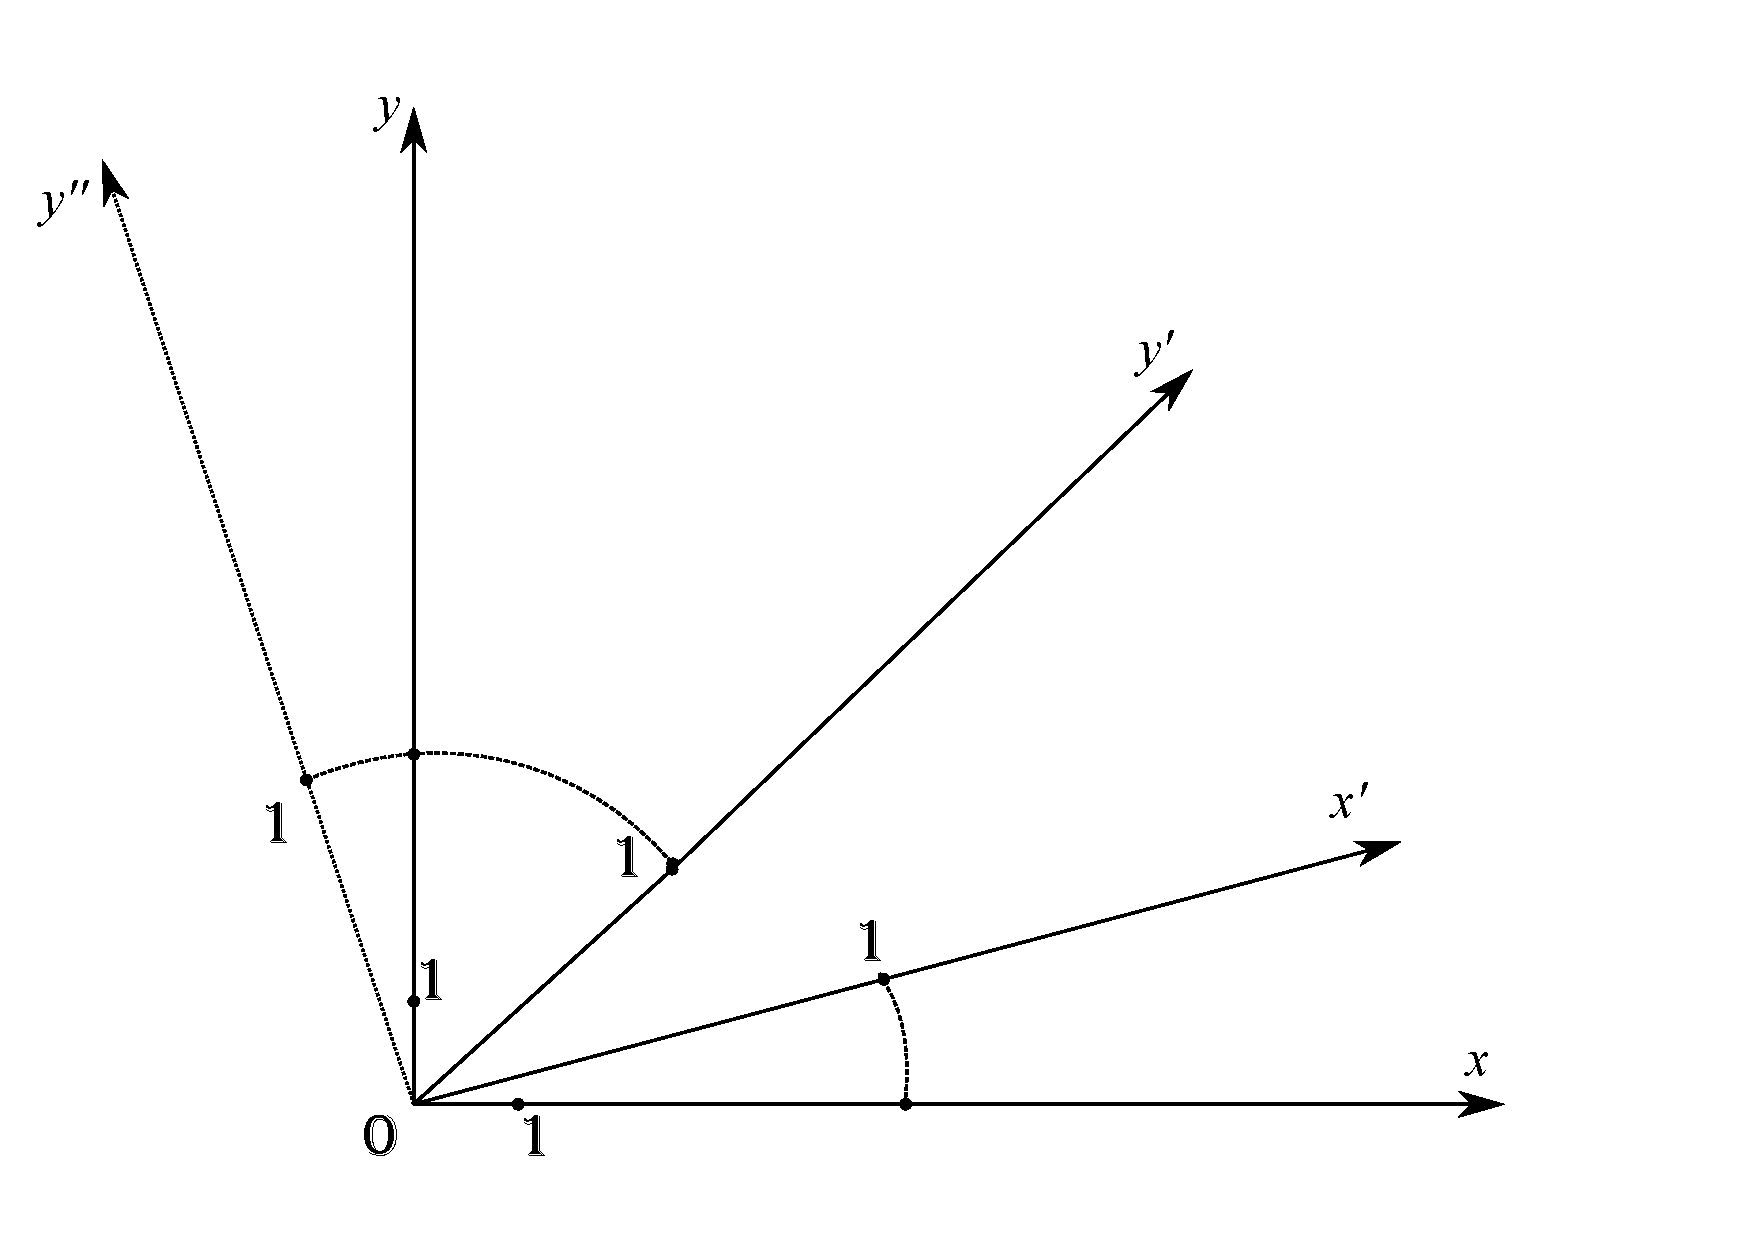
\includegraphics[width=\textwidth]{33_01}}{Это демонстрируется рисунком справа.
Здесь сначала произведено масштабирование, затем поворот, а потом сдвиг. Новая
система координат \( (x', y') \) является косоугольной.

Важную роль в физике играет понятие \emph{тензора} (в частном случае
\emph{вектора} или \emph{скаляра}). Изначально тензоры появились при описании
геометрических объектов - поверхностей \( n \)-го порядка в трёхмерном
пространстве.
}

Так плоскость - поверхность 1-го порядка - в декартовых координатах
\( (x, y, z) \), задаётся 4 числами - вектором \( \{a,b,c\} \) (тензором
первого ранга) и скаляром \( d \):
\[
    ax+by+cz+d=0.
\]

\emph{Тензором \( n \)-го ранга} называется система занумерованных величин,
которая преобразуется при линейных преобразованиях координат определённым
образом (если мы дали определение вектора и тензорного произведения -- как
тензорное произведение \( n \)-векторов с учётом их ко- и контр- вариантности).
Тензором нулевого ранга называется скаляр.

Будем понимать под вектором направленный отрезок. Суммирование векторов будем
проводить по правилу параллелограмма. Тройку некомпланарных (не лежащих в одной
плоскости) векторов будем называть базисом. Модуль (длину) вектора определять
как длину отрезка. Векторы единичной длины называть ортами. Для обозначения
тройки будем использовать индексы, например, \( \vec{e}_{i} \) это три вектора
\( \vec{e}_{1} \), \( \vec{e}_{2} \), \( \vec{e}_{3} \), \( x_i \) - три
величины \( x_1 \), \( x_2 \), \( x_3 \). В качестве индексов использовать
буквы \( i \), \( j \), \( k \), \( \ldots \) . Считать, что каждый вектор
раскладывается по данному базису единственным образом, скалярное произведение
определять по стандартной формуле
\[
    \vec{a}\cdot\vec{b} = |\vec{a}||\vec{b}|\cos (\widehat{\vec{a}\vec{b}}).
\]
Для записи сумм использовать \emph{правило Эйнштейна} - вести суммирование по
повторяющимся индексам.

Векторы в данном базисе могут быть определены ковариантным или контрвариантным
образом. Поясним смысл контр- и ко- вариантности. На плоскости зададим
неортогональный базис из ортов \( \vec{e}_{1} \) и \( \vec{e}_{2} \) как
показано на рисунке.

\sidefig(9cm)
{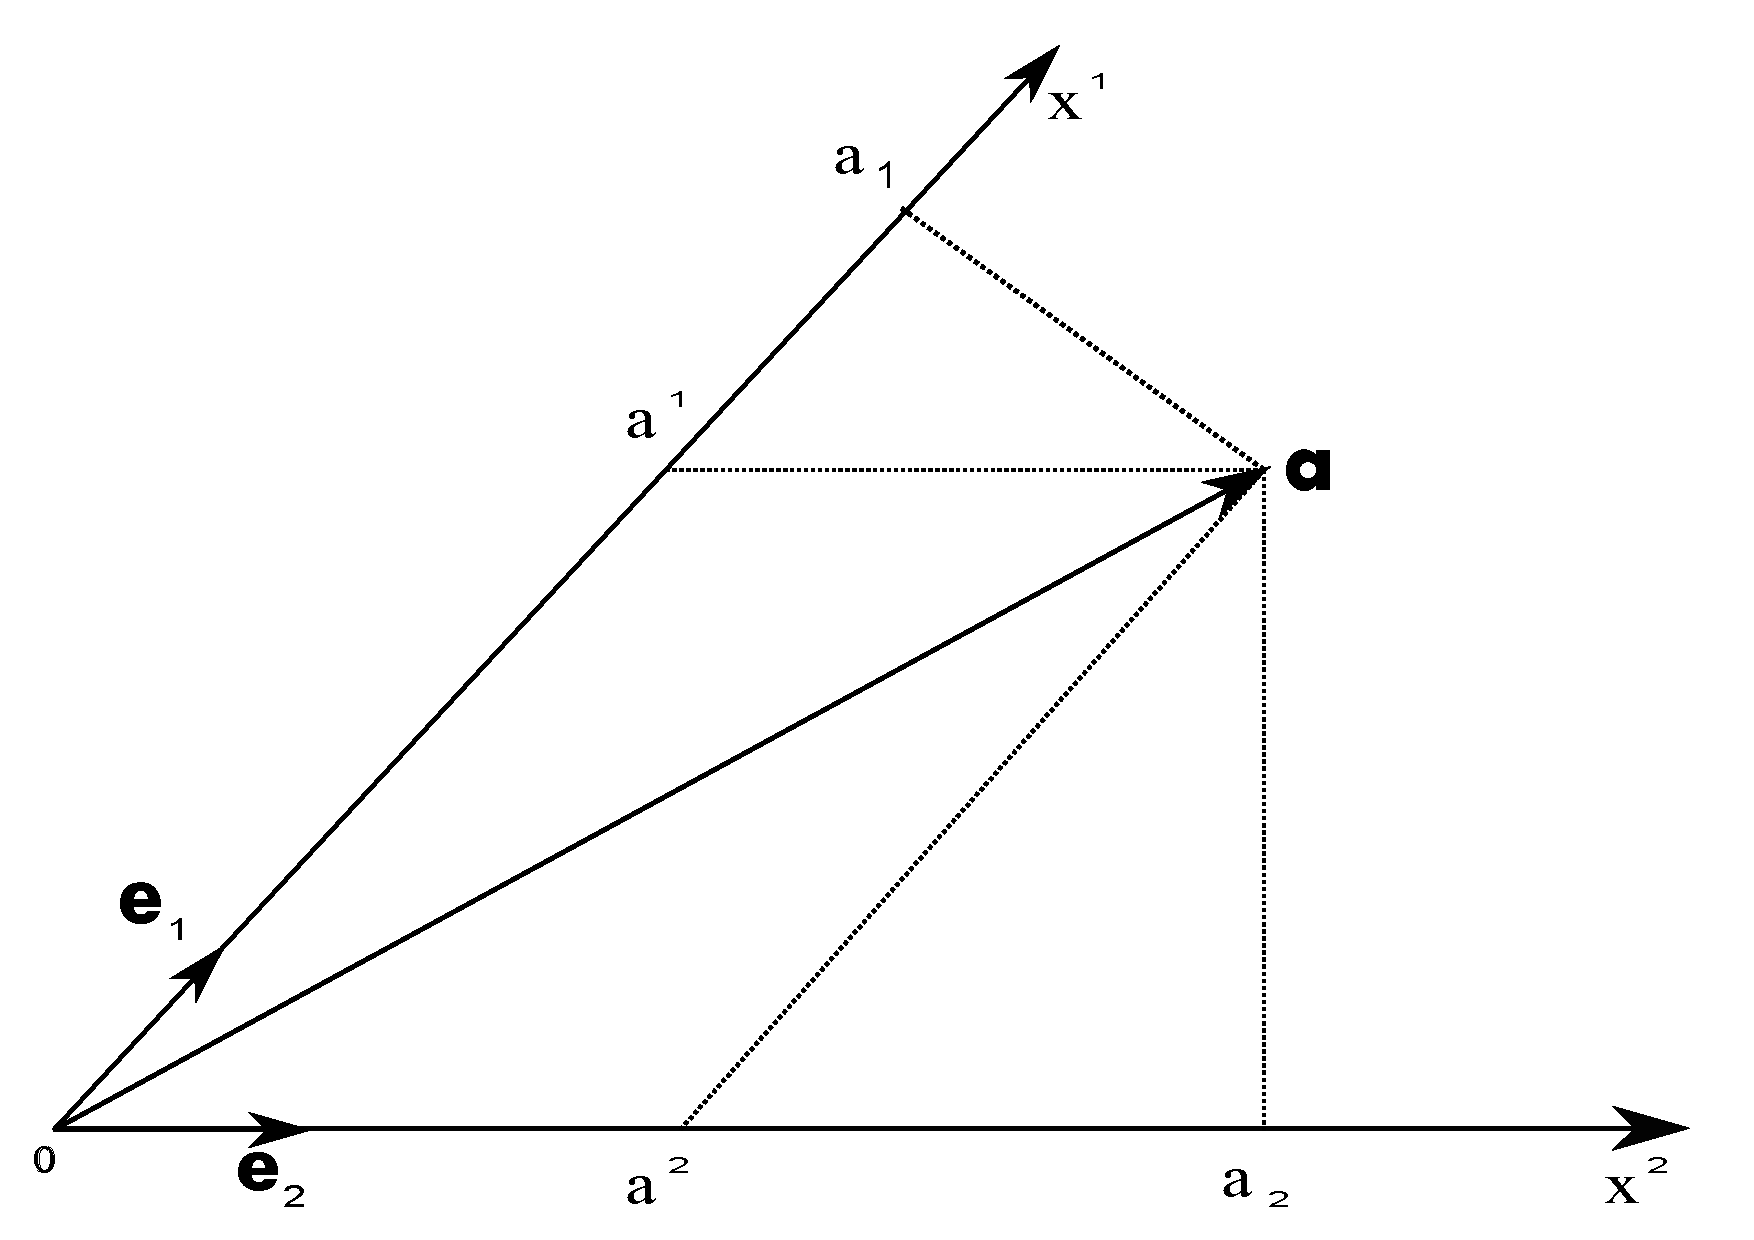
\includegraphics[width=\textwidth]{33_02}}{
Проекции вектора \( \vec{a} \) на орты \( \vec{e}_{1} \) и \( \vec{e}_{2} \)~--
\( a_1 \)  и \( a_2 \) называются \emph{ковариантными} компонентами, а
коэффициенты в разложении по базису \( \vec{e}_{1} \) и \( \vec{e}_{2} \)~--
\( a^1 \)  и \( a^2 \):
\[
    \vec{a} = a^1 \vec{e}_{1} + a^2 \vec{e}_{2} \text{ -- }
\]
\emph{контрвариантными} компонентами. Для ковариантных компонент можно
построить базис из векторов \( \vec{e}^{1} \) и \( \vec{e}^{2} \),
называемый \emph{взаимным} или \emph{биортогональным}.}

В этом базисе вектор \( \vec{a} \) можно разложить по ковариантным компонентам:
\[
    \vec{a} = a_1 \vec{e}^{1} + a_2 \vec{e}^{2}.
\]
    
В общем случае тройка некомпланарных векторов \( \vec{e}_{1} \),
\( \vec{e}_{2} \) и \( \vec{e}_{3} \) образует базис. Базис \( \vec{e}^{1} \),
\( \vec{e}^{2} \), \( \vec{e}^{3} \) связанный с \( \vec{e}_{1} \),
\( \vec{e}_{2} \), \( \vec{e}_{3} \) соотношением:
\[
    \vec{e}^{i}\cdot\vec{e}_{j} = \delta^i_{j}
\]
называется \emph{взаимным} или \emph{биортогональным}(\( \delta^i_{j} \) --
символ Кронекера).  Коэффициенты разложения вектора \( \vec{a} \) по базису
\( \vec{e}_{i} \) носят название \emph{контрвариантных} компонент вектора и
обозначаются \( a^i \), а по базису \( \vec{e}^{i} \) носят название
\emph{ковариантных} компонент и обозначаются \( a_i \). Для ортонормированного
базиса (в декартовой системе координат) ковариантные и контрвариантные
компоненты и базисы совпадают.
    
Найдём закон преобразования компонент вектора \( \vec{a} \) при переходе от
одного базиса к другому. Обозначим компоненты \( \vec{a} \) в новом базисе
\( \vec{e}_y{'}_{i} \) - \( \alpha^i \), в старом базисе \( \vec{e}_{i} \) -
\( a^i \). Тогда
\begin{gather*}
    \vec{a} = \alpha^i\vec{e}_y{'}_{i} = a^i\vec{e}_{i}, \\
    \alpha^i \vec{e}_y{'}_{i}\cdot \vec{e}_y{'}^{j} = \alpha^i \delta_{ij} =
    \alpha^j = a^i\vec{e}_{i}\cdot \vec{e}_y{'}^{j} = \gamma_i{}^j a^i,
\end{gather*}
где обозначено \( \gamma_i{}^j = \vec{e}_{i}\cdot \vec{e}_y{'}^{j} \).
Аналогично можно получить:
\begin{gather*}
    \alpha_j =
    \gamma_{ij} a^i,~~
    \alpha^j =
    \gamma^{ij} a_i,~~
    \alpha_j =
    \gamma^i{}_j  a_i, \\
    \gamma_{ij} = \vec{e}_{i}\cdot \vec{e}_y{'}_{j},~~
    \gamma^{ij} = \vec{e}^{i}\cdot \vec{e}_y{'}^{j},~~    
    \gamma^i{}_j = \vec{e}^{i}\cdot \vec{e}_y{'}_{j}.
\end{gather*}
    
Компоненты тензоров также можно определять ковариантным или контрвариантным
 образом. Так например тензор второго ранга \( a \) с компонентами:
\begin{itemize}
    \item \( a_{ij} \) задан ковариантными компонентами;
    \item \( a^{ij} \) задан контрвариантными компонентами;
    \item \( a^i{}_j \) задан смешанными компонентами.
\end{itemize}

Для тензоров справедливы операции:
\begin{itemize}
    \item \emph{сложение} - тензоры одинакового ранга с одинаково заданными
    компонентами можно складывать: \( a_i + b_i = c_i \); результатом сложения
    является тензор того же ранга, что и исходные;
    \item \emph{умножение} - любые два тензора можно перемножить:
    \( a_{ij}b^k{}_l = c_{ij}{}^k{}_l \); результатом умножения является тензор
    рангом равным сумме рангов  исходных тензоров, ковариантность,
    контрвариантность сохраняется, при этом порядок компонент очень важен;
    \item \emph{свёртка} - любой тензор можно свернуть по ковариантному и
    контрвариантному индексам: \( c_{ik}{}^k{}_l = d_{il}  \); результатом
    свёртки является тензор, ранг которого меньше на два, чем ранг исходного
    тензора.
\end{itemize}   

Это позволяет точно записать закон преобразования компонент тензора, например,
для тензора \( a \) второго ранга с ковариантными компонентами
\[
    a'_{ij} = \gamma^k{}_i\ \gamma^l{}_j\ a_{kl}
\]
 или для тензора \( a \) четвёртого  ранга со смешанными компонентами
\[
    a'_{ij}{}^{k}{}_{l} = \gamma^m{}_i\ \gamma^n{}_j\ 
    \gamma_p{}^k\ \gamma^v{}_l\ a_{mn}{}^{p}{}_{v}.
\]  

Тензоры \( g^{ij} = \vec{e}^{i} \cdot \vec{e}^{j} \) и
\( g_{ij} = \vec{e}_{i} \cdot \vec{e}_{j} \) носят название
\emph{фундаментальных метрических} тензоров. Они возникают при поиске
скалярного произведения двух векторов \( \vec{a} \) и \( \vec{b} \)
\[
    \vec{a}\cdot\vec{b} = g_{ij} a^i b^j = g^{ij} a_i b_j,
\]
при поиске модуля вектора \( \vec{a} \)
\[
    |\vec{a}|^2 = \vec{a}\cdot\vec{a} =
    g_{ij}a^ia^j = g^{ij} a_i a_j
\]
и характеризует метрику пространства (расстояние между двумя близкими точками в
координатах \( x^i \))
\[
    ds^2 = g_{ij}dx^idx^j = g^{ij} dx_i dx_j.
\]      
В прямоугольных декартовых координатах:
\[
    g_{ij} = g^{ij} =
        \left(
            \begin{array}{ccc}
            1 & 0 & 0 \\
            0 & 1 & 0 \\
            0 & 0 & 1
            \end{array}
        \right).
\]
    
Задать криволинейные координаты - значит задать свой базис в каждой точке
пространства (\emph{подвижный базис}), этот базис будет задан контрвариантным
образом для ковариантных криволинейных координат и ковариантным образом для
контрвариантных криволинейных координат. Обозначим контрвариантные
криволинейные координаты \( q^i \), базис выберем в виде векторов
\( \vec{e}_{i} \) касательных к координатным линиям. Радиус-вектор от начала
координат до данной точки сложным образом зависит от криволинейных координат:
\[
    \vec{r} = \vec{r}(q^1, q^2, q^3).
\]
Дифференциал радиус-вектора \( \vec{r} \):
\[
    d\vec{r} = \pder{\vec{r}}{q^i}dq^i.
\]
Учитывая, что вдоль координатной линии две координаты из трёх постоянны в
качестве базиса можно выбрать
\[
    \vec{e}_{i} =  \pder{\vec{r}}{q^i}.
\]
    
Фундаментальный метрический тензор теперь зависит от координат и позволяет
определять только расстояние между двумя близкими точками:
\[
    ds^2 = d\vec{r}\cdot d\vec{r} = 
    \pder{ \vec{r}}{q^i}\cdot \pder{ \vec{r}}{q^j} dq^i dq^j =
    g_{ij} dq^i dq^j.
\]

Докажем одно свойство фундаментального метрического тензора. Определяя вектор
\( \vec{a} \) в криволинейных координатах как контрвариантных, так и
ковариантных в данной точке 
\[
    a_i \vec{e}^{i} =  a^i \vec{e}_{i}
\]
и домножая скалярно на орт \( \vec{e}_{j} \), получим
\[
    a_j = a^i g_{ij}.
\]
Далее рассмотрим выражение:
\[
    a_j a^j = g_{ij} g^{jk} a^i a_k = a^2 = \delta^k_i a^i a_k,
\]
где \( \delta^k_i \) - символ Кронекера. А так как \( a^i a_k \) линейно
независимы, то 
\[
    g_{ij} g^{jk}= \delta^k_i.
\]


Для криволинейных ортогональных координат базисные орты:
\[
    \vec{e}_{i} = \frac{1}{H_i} \pder{ \vec{r}}{q^i}\text{ (по \( i \)
    суммирования нет)}
\]
где \( H_i \) - коэффициенты Ламе, тогда \( g \):
\[
    g_{ij}  =
        \left(
            \begin{array}{ccc}
            H_1^2 & 0 & 0 \\
            0 & H_2^2 & 0 \\
            0 & 0 & H^2_3
            \end{array}
        \right).
\]
Так, например:
\begin{itemize}
    \item в цилиндрических координатах \( (r,\varphi,z) \):
\[
    g_{ij}  =
        \left(
            \begin{array}{ccc}
            1 & 0 & 0 \\
            0 & r^2 & 0 \\
            0 & 0 & 1
            \end{array}
        \right);
\]

    \item в сферических координатах \( (r,\theta, \varphi) \):
\[
    g_{ij}  =
        \left(
            \begin{array}{ccc}
            1 & 0 & 0 \\
            0 & r^2 & 0 \\
            0 & 0 & r^2 \sin^2 \theta
            \end{array}
        \right).
\]
\end{itemize}
\newpage
